\documentclass[conference,onecolumn,brazilian]{IEEEtran}
%\IEEEoverridecommandlockouts

\usepackage[utf8]{inputenc}
\usepackage[brazilian]{babel}
\usepackage{cite}
\usepackage{amsmath,amssymb,amsfonts}
\usepackage{algorithmic}
\usepackage{graphicx}
\usepackage{textcomp}
\usepackage{xcolor}
\usepackage{hyperref}
\usepackage{cleveref}
\usepackage{longtable}

\def\BibTeX{{\rm B\kern-.05em{\sc i\kern-.025em b}\kern-.08em
    T\kern-.1667em\lower.7ex\hbox{E}\kern-.125emX}}
\begin{document}

\newcommand{\ant}{\textsc{Ant Colony Optmization}} 
\newcommand{\nomeprograma}{Sistema de acasalamento}

\newtheorem{definition}{Definição}

\title{Um estudo sobre meta-heurística: Ant Colony Optimization}

\author{\IEEEauthorblockN{1\textsuperscript{st} Thálys Lemos Correa}
\IEEEauthorblockA{\textit{Engenharia de Computação -- Campus Bagé} \\
\textit{Universidade Federal do Pampa}\\
thalyscorrea.aluno@unipampa.edu.br}
\and
\IEEEauthorblockN{2\textsuperscript{nd} Vitor da Silva Ferreira}
\IEEEauthorblockA{\textit{Engenharia de Computação -- Campus Bagé} \\
\textit{Universidade Federal do Pampa)}\\
vitordsf.aluno@unipampa.edu.br}
}

\maketitle

\begin{abstract}
Este trabalho apresenta a aplicação da meta-heurística \textit{Ant Colony System} (ACS) para resolver o problema de acasalamento otimizado em rebanhos bovinos, visando simultaneamente minimizar a coancestralidade entre os descendentes e maximizar o ganho genético esperado. O problema é modelado como um grafo bipartido que conecta machos e fêmeas, no qual cada aresta representa uma possível combinação de acasalamento ponderada por feromônios e heurísticas genéticas. A implementação proposta realiza pré-processamento dos dados, indexação eficiente da coancestralidade e construção de soluções probabilísticas respeitando restrições reprodutivas, como o limite máximo de uso dos machos. Experimentos conduzidos com diferentes limites de acasalamento demonstraram que valores mais altos tendem a aumentar o ganho genético, mas também elevam significativamente a coancestralidade. A normalização dos critérios e a aplicação de uma função de utilidade permitiram identificar o melhor equilíbrio entre os objetivos conflitantes, que neste estudo ocorreu com o limite de 15 acasalamentos por macho. Os resultados confirmam a adequação do ACS para decisões multicritério em manejo genético, oferecendo soluções eficientes e biologicamente plausíveis.
\end{abstract}
\vspace{1em}

\begin{abstract}
This work applies the \textit{Ant Colony System} (ACS) metaheuristic to solve the optimized mating problem in cattle herds, aiming simultaneously to minimize coancestry among offspring and to maximize expected genetic gain. The problem is modeled as a bipartite graph connecting males and females, where each edge represents a possible mating combination weighted by pheromones and genetic heuristics. The proposed implementation performs data preprocessing, efficient coancestry indexing, and probabilistic solution construction while respecting reproductive constraints such as the maximum usage limit of each male. Experiments conducted under different mating limits show that higher limits tend to increase genetic gain but also significantly raise coancestry. Normalization of the criteria and the use of a utility function enabled identifying the best balance between the conflicting objectives, which in this study occurred at a limit of 15 matings per male. The results confirm the suitability of ACS for multicriteria decision-making in genetic management, providing efficient and biologically meaningful solutions.
\end{abstract}

\begin{IEEEkeywords}
Ant Colony System, Otimização Combinatória, Coancestralidade, Melhoramento Genético, Problema de Acasalamento, Meta-heurísticas.
\end{IEEEkeywords}

\section{Introdução}
Algoritmos de Colônias de Formigas, ou \textit{Ant Colony Optimization} (ACO), constituem uma classe de meta-heurísticas amplamente utilizada na resolução de problemas de otimização combinatória, especialmente naqueles cuja solução exata é computacionalmente intratável \cite{dorigo2018introduction}. Esses métodos são inspirados no comportamento observado em colônias de formigas reais, particularmente no uso de feromônios como forma de comunicação indireta. Na natureza, as formigas reforçam trajetos vantajosos ao depositar feromônios ao longo do caminho, permitindo que outras formigas identifiquem rotas promissoras. Com isso, caminhos ineficientes tendem a ser descartados, enquanto rotas mais produtivas são naturalmente privilegiadas.

Com base nesse princípio, algoritmos ACO constroem soluções por meio da cooperação de formigas artificiais, agentes simples guiados por regras locais. O processo é assíncrono, probabilístico e estruturado de forma a reduzir a chance de estagnação em ótimos locais. A solução é representada como um grafo que descreve a combinação de estados que maximiza o desempenho segundo a função objetivo. Esse paradigma foi formalizado por Marco Dorigo em sua tese de doutorado (1992), que introduziu o \textit{Ant System}, posteriormente aprimorado em variantes como o \textit{MAX-MIN Ant System} \cite{stutzle2000max} e o \textit{Ant Colony System} \cite{dorigo2002ant}.

Neste contexto, o presente trabalho tem como objetivo aplicar a meta-heurística Ant Colony System (ACS) à resolução de um problema de acasalamento otimizado no qual se busca minimizar os riscos associados a cruzamentos consanguíneos e maximizar a o valor genético esperado da prole. Diferentemente da Ant System clássica de Dorigo, a ACS aplica feromônios a cada passo, o que aumenta a diversificação da busca durante a construção de soluções, realizando atualização global apenas nas melhores soluções ao final de cada iteração, equilibrando a exploração de novos caminhos e o aprofundamento no desenpenho de caminhos promissores \cite{dorigo2002ant}.

Relações de parentesco elevadas tendem a gerar descendentes mais suscetíveis a problemas de saúde física e reprodutiva, tornando necessário controlar a estrutura genética do rebanho ao longo das gerações. Embora o melhor macho do rebanho possa, em princípio, maximizar o valor econômico da prole, seu uso repetido cria descendentes altamente aparentados, o que inviabiliza a sustentabilidade das gerações futuras sem introdução de novos animais. Para quantificar o parentesco entre os indivíduos, utilizamos a medida de coancestralidade, uma relação que identifica o grau de compartilhamento de ancestrais entre dois animais e permite estimar o potencial de consanguinidade nos descendentes. Assim, o método proposto integra princípios de otimização por colônias de formigas com fundamentos de genética quantitativa, visando construir estratégias de acasalamento que atendam simultaneamente ao desempenho produtivo e à saúde genética do rebanho.
\section{Caracterização e complexidade do problema}
\label{sec-complexidade-problema}
Sejam \(M\) o conjunto de machos (touros) e \(F\) o conjunto de fêmeas (vacas). Para cada par \((i,j)\), com \(i\in M\) e \(j\in F\), definimos a variável de decisão binária 
\[ x_{i,j} = \begin{cases} 1, & \text{se a fêmea } j \text{ for cruzada com o macho } i,\\[4pt] 0, & \text{caso contrário.} \end{cases} \]
A função objetivo consiste em minimizar a coancestralidade total entre os descendentes gerados:
\[ \min\; P(x) = \sum_{(x,y)}\sum_{(w,v)} c_{(x,y)(w,v)} \; x_{x,y}\, x_{w,v}, \] 
onde \(c_{(x,y)(w,v)}\in[0,1]\) representa o coeficiente de coancestralidade entre os descendentes dos casais \((x,y)\) e \((w,v)\). As restrições do modelo são:
\begin{enumerate} 
    \item \textbf{Cada fêmea cruza exatamente uma vez:} \[ \forall j\in F:\quad \sum_{i\in M_j} x_{i,j} = 1, \] onde \(M_j\subseteq M\) denota o subconjunto de machos compatíveis com a fêmea \(j\). 
    \item \textbf{Limite de usos por macho:} \[ \forall i\in M:\quad \sum_{j\in F} x_{i,j} \le U_i, \] com \(U_i\) definindo o número máximo de cruzamentos permitidos para o macho \(i\) (por exemplo, \(U_i\in\{12,18,20\}\) nos cenários testados). 
    \item \(\,x_{i,j}\in\{0,1\}\) para todo \(i\in M, j\in F\). 
\end{enumerate} 
Em resumo, o problema pode ser formulado como um problema de otimização combinatória binária: 
\[ \begin{aligned} 
\min\quad & P(x) = \sum_{(x,y)}\sum_{(w,v)} c_{(x,y)(w,v)} \, x_{x,y}\, x_{w,v}\\ 
\text{sujeito a:}\quad & \sum_{i\in M_j} x_{i,j} = 1\quad \forall j\in F,\\
&\sum_{j\in F} x_{i,j} \le U_i\quad \forall i\in M,\\
& x_{i,j}\in\{0,1\}. 
\end{aligned} \]

No contexto da ACS, o problema de acasalamento é reinterpretado como um grafo bipartido que conecta o conjunto de fêmeas \(F\) ao conjunto de machos \(M\), onde cada aresta \((i,j)\) do grafo representa uma decisão possível de acasalamento entre o macho \(i\) e a fêmea \(j\), associada a um nível de feromônio \(\tau_{i,j}\) que indica a atratividade acumulada daquela combinação com base em iterações anteriores. 

Além do feromônio, define-se uma heurística de visibilidade \(\eta_{i,j}\) construída a partir dos índices genéticos dos animais, permitindo favorecer combinações com maior potencial genético. 
Cada formiga percorre o grafo selecionando, para cada fêmea, um macho válido por meio de uma regra probabilística que combina o feromônio acumulado e a heurística genética. A probabilidade de escolha é proporcional a \(\tau_{i,j}^{\alpha}\eta_{i,j}^{\beta}\), de modo que tanto a experiência da colônia quanto a qualidade local da decisão influenciam o processo, sempre em conformidade com as restrições do problema.
Após a construção de cada solução, o ACS realiza tanto atualizações locais quanto globais do feromônio, permitindo equilibrar exploração e intensificação e conduzindo a busca a soluções de menor parentesco.


\section{Algoritmo X (nome do algoritmo da solução)}
\label{sec-complexidade-algoritmo}

Nesta seção são descritas as etapas da ACS aplicado ao problema anteriormente apresentado, foi utilizado a ferramenta \textit{Google Colab} para a implementação do código em \textit{Python} por permitir o desenvolvimento simultâneo de dois desenvolvedores, o que favore. Para facilitar a implementação do algoritmo, decidiu-se organizá-lo da seguinte forma:
\begin{enumerate}
    \item Importação e inicialização;
    \item Construção da solução por cada formiga naquela iteração;
    \item Calculo de custo de coancestralidade;
    \item Calculo de valor genético dos animais;
    \item Atualização da melhor solução encontrada;
    \item Evapora e deposita os feromônios conforme o desempenho das soluções;
\end{enumerate}
\vspace{1em}

\subsection*{1) Inicialização e Preparação das Estruturas}
Esse trecho de código implementa a primeira etapa do processo, responsável por carregar, validar e padronizar os arquivos de entrada utilizados pelo algoritmo ACS. Inicialmente, são importadas bibliotecas essenciais para manipulação de dados, operações matemáticas, controle de arquivos e entrada do usuário. Em seguida, o código lê automaticamente o arquivo contendo informações de coancestralidade diretamente de uma URL do \textit{GitHub}, normaliza seus nomes de colunas e garante que elas sigam o formato padrão esperado pelo algoritmo. Esse processo inclui tratamento de erros e  detecção de suporte ao ambiente utilizado. Após a seleção, o arquivo é lido com segurança; caso a leitura falhe, o programa é encerrado para evitar inconsistências futuras. Por fim, as colunas do arquivo de índices são padronizadas, convertendo nomes para minúsculas, removendo espaços e renomeando-as para os identificadores esperados. Essa padronização garante que, independentemente da origem ou formatação original do arquivo, os dados estarão consistentes para as etapas seguintes do algoritmo.

\begin{verbatim} 
start_time = time.time()

para iteracao em 0 .. NUM_ITERACOES:
    criar lista solutions_in_iteracao
    para cada formiga:
        caminho_formiga = []
        uso_machos = dicionario contador zerado
        valid_path = True
\end{verbatim}
\vspace{1em}

\subsection*{2) Construção da Solução por Cada Formiga}
Essa etapa identifica automaticamente os machos e fêmeas presentes nos dados de coancestralidade. Para isso, cada código no formato machoID\_femeaID é dividido para extrair separadamente os identificadores, que são armazenados em conjuntos para garantir unicidade. Após processar todas as entradas, os conjuntos são convertidos em listas ordenadas, permitindo determinar o número total de machos e fêmeas utilizados no problema.

\begin{verbatim}
para cada fêmea i_f:
    probabilidades = []
    candidatos_validos = []

    para cada macho i_m:
        se uso_machos[i_m] >= MAX_USO_MACHO:
            prob = 0
        senao:
            t = tau[i_f, i_m] ** ALPHA
            n = heuristica[i_f, i_m] ** BETA
            prob = t * n
            adicionar i_m a candidatos_validos

        armazenar prob nas probabilidades

    denom = soma(probabilidades)

    se denom > 0:
        normalizar probabilidades
        escolha_macho_idx = escolha aleatória ponderada
    senao:
        se candidatos_validos vazio: descartar caminho
        escolha_macho_idx = escolha aleatória simples

    registrar (i_f, escolha_macho_idx) no caminho
    incrementar uso_machos[escolha_macho_idx]
\end{verbatim}
\vspace{1em}

\subsection*{3) Cálculo da Coancestralidade da Solução}
A etapa de cálculo da coancestralidade tem como objetivo transformar os dados brutos presentes no dataframe em uma matriz (ou estrutura equivalente) que permite consultar rapidamente o coeficiente de parentesco entre qualquer par macho–fêmea. Embora o trecho de código não tenha sido mostrado, o funcionamento típico dessa fase — e o papel que ela cumpre dentro do algoritmo — pode ser descrito da seguinte forma:

\begin{verbatim}
cost_coancestralidade = 0
pares_reais = converter índices (i_f, i_m) para (id_m, id_f)

para i em 0..n_pares:
    para j em i+1 .. n_pares:
        cost += coancestralidade_dict[(par_i, par_j)]
\end{verbatim}
\vspace{1em}

\subsection*{4) Cálculo da Soma dos Índices Genéticos}
Esta etapa calcula a partir dos índices genéticos de machos e fêmeas. Primeiro, os índices individuais são extraídos e combinados em todas as possíveis duplas macho–fêmea, somando cada par e dividindo por dois para obter um valor médio representativo. Em seguida, a matriz resultante é verificada para identificar valores zero ou negativos, que prejudicariam o comportamento do ACO; caso existam, toda a matriz é normalizada ao adicionar o módulo do menor valor mais 1, garantindo que todos os elementos sejam positivos. O resultado final é armazenado que será utilizada como componente heurística na construção das soluções pelas formigas.

\begin{verbatim}
sum_indice_genetico = 0

para cada par (i_f, i_m) no caminho:
    sum_indice_genetico += matriz_indices_reais[i_f, i_m]
\end{verbatim}
\vspace{1em}

\subsection*{5) Atualização da Melhor Solução Global}
Esta etapa transforma os dados brutos de coancestralidade em uma estrutura eficiente para consulta e coleta um parâmetro essencial do ACO. Primeiro, cada identificação no formato macho\_fêmea é convertida em uma tupla numérica, e um dicionário é criado para armazenar rapidamente o coeficiente de coancestralidade entre qualquer par de casais — incluindo ambas as ordens, garantindo acesso simétrico. Esse dicionário será usado pelo algoritmo para calcular o impacto genético das combinações durante a otimização. Em seguida, o código apresenta um menu simples para que o usuário escolha o limite máximo de uso dos machos, definindo uma das principais restrições do problema antes de iniciar o processo de busca do ACO.

\begin{verbatim}
se cost < best_cost:
    atualizar best_cost
    atualizar best_solution
    atualizar best_index_sum

senao se cost == best_cost e sum_indice_genetico > best_index_sum:
    atualizar best_solution e índices
\end{verbatim}
\vspace{1em}

\subsection*{6) Evaporação e Deposição de Feromônio}
Esse trecho implementa o núcleo do algoritmo de Otimização por Colônia de Formigas responsável por buscar a melhor combinação entre machos e fêmeas. O processo começa inicializando parâmetros como número de formigas, iterações, importância do feromônio \(\alpha\) , da heurística \(\beta\)\, taxa de evaporação e matriz de feromônios. A cada iteração, cada formiga constrói uma solução completa escolhendo um macho para cada fêmea com base em probabilidades que dependem tanto do feromônio acumulado quanto da heurística genética sempre respeitando o limite de uso dos machos. Ao final de cada construção, a solução é avaliada por dois critérios: minimizar a coancestralidade e maximizar o índice genético total. A melhor solução encontrada é mantida, e os feromônios são atualizados: evaporam globalmente e aumentam proporcionalmente à qualidade das soluções construídas. Esse ciclo se repete por várias iterações, guiando gradualmente o algoritmo para combinações mais promissoras até alcançar a melhor configuração encontrada dentro do número definido de iterações.

\begin{verbatim}
tau *= (1 - EVAPORATION)

para cada solucao em solutions_in_iter:
    custo = sol[custo]
    se custo <= 0.0001: custo = 0.0001
    delta = Q / custo

    para cada par (i_f, i_m) da solução:
        tau[i_f, i_m] += delta
\end{verbatim}
\vspace{1em}

\subsection*{7) Impressão dos Resultados e Relatório Final}
Essa etapa é responsável por apresentar e validar o resultado final encontrado pelo algoritmo ACO. Primeiro, o código percorre a melhor solução identificada, reconstrói cada par fêmea–macho e calcula o índice genético correspondente, armazenando tudo em uma lista organizada para análise. Ele imprime apenas os dez primeiros pares para visualização, informando caso haja mais resultados. Em seguida, contabiliza quantas vezes cada macho foi usado e calcula estatísticas finais importantes: custo mínimo de coancestralidade, soma total dos índices genéticos, média dos índices da progênie e o macho mais utilizado. Por fim, verifica se a restrição de uso máximo por macho foi respeitada e informa o status geral da solução; caso nenhuma solução tenha sido encontrada, exibe um aviso de falha crítica.

\begin{verbatim}
end_time = time.time()
print("Tempo total:", end_time - start_time)

se best_solution existe:
    para cada par (i_f, i_m) na solução:
        imprimir IDs e índice genético

    gerar estatísticas gerais:
        - melhor custo
        - soma de índices
        - média da prole
        - machos mais usados
        - verificação da restrição de uso

senao:
    imprimir "FALHA CRÍTICA: Nenhuma solução encontrada."
\end{verbatim}

Após a implementação do algoritmo foi realizado uma análise para avaliar o custo dominante da análise assintótica, onde foi evidenciado dois custos principais:
\begin{itemize}
    \item Cálculo da coancestralidade, onde a cada iteração o custo é \(O((i\_j)^2)\);
    \begin{verbatim}
        for i in range(n_pares):
            for j in range(i + 1, n_pares):
                coancest_dict += coancest_dict.get((par_a, par_b), 0.0)
    \end{verbatim}
    \item Custo de construir o caminho da formiga, onde para cada fêmea é avaliado um macho, construindo um custo de \(O(i\ *\ j)\), que, dependendo do contexto, pode vir a ser \(O((i\_j)^2)\) dependendo do número de formigas.
    \begin{verbatim}
        for i_f in range(num_femeas):
            probabilidades = []
            candidatos_validos = []

            for i_m in range(num_machos):
                if uso_machos[i_m] >= MAX_USO_MACHO:
                prob = 0.0
            else:
                t = tau[i_f, i_m] * ALPHA
                n = matriz_heuristica_eta[i_f, i_m] * BETA
                prob = t * n
                candidatos_validos.append(i_m)
            probabilidades.append(prob)
    \end{verbatim}
\end{itemize}
Dessa forma, é possível observar que a complexidade final do algoritmo também deve incluir \(I\) iterações e \(n\) formigas, além dos \(i\_j\)\ pares, assim, o custo total leva em conta é :

\begin{center}
    \(O(I\ *\ A\ *\ (n^2\ +\ i\ *\ j))\)
\end{center} 
Que pode ser simplificado em, considerando que o termo dominante do parêntese é o \(n^2\):
\begin{center}
    \(O(I\ *\ A\ *\ n^2)\)
\end{center}
\vspace{1em}
\section{Análise de Complexidade Experimental}

Além da análise teórica da complexidade, foi conduzida uma avaliação empírica do custo computacional do algoritmo ACO. Para isso, variou-se isoladamente o número de formigas e o número de iterações, registrando-se o tempo total de execução em cada configuração. É importante destacar que esses gráficos não representam a convergência do algoritmo, mas sim sua escalabilidade temporal.

A Figura~\ref{fig:tempo_formigas} apresenta a relação entre o tempo de execução e o tamanho da população de formigas. Observa-se um crescimento aproximadamente linear, o que confirma o comportamento esperado da complexidade, uma vez que cada formiga constrói uma solução completa em cada iteração. Assim, aumentar o número de formigas aumenta diretamente o custo computacional.

\begin{figure} [htpb]
    \centering
    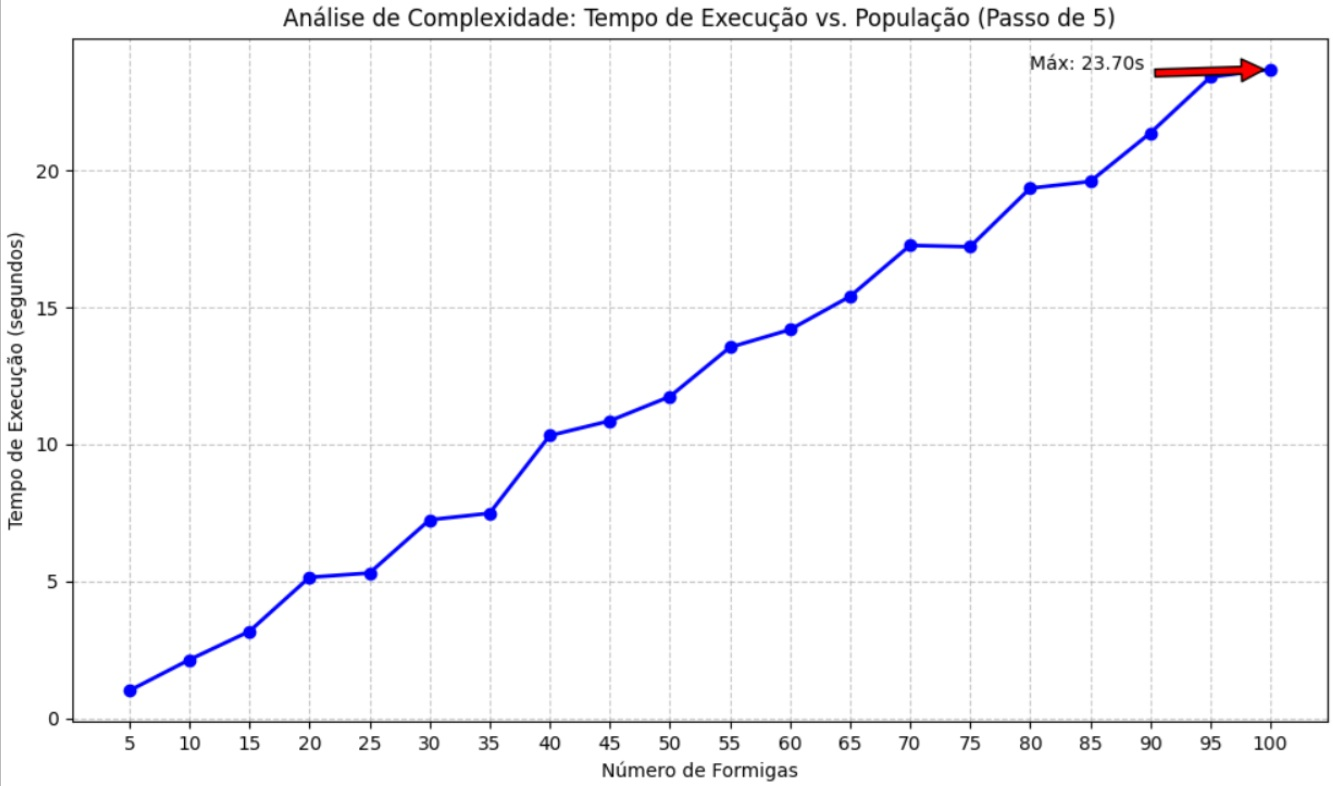
\includegraphics[width=0.75\linewidth]{Imagens/num_formigas.jpg}
    \caption{Tempo de execução em função do número de formigas.}
    \label{fig:tempo_formigas}
\end{figure}

Já a Figura~\ref{fig:tempo_iteracoes} mostra o tempo de execução em função do número de iterações. Também se verifica crescimento linear, uma vez que cada iteração envolve a construção de todas as soluções e a atualização global dos feromônios. Portanto, o custo cresce proporcionalmente ao número de ciclos da colônia.

\begin{figure} [htpb]
    \centering
    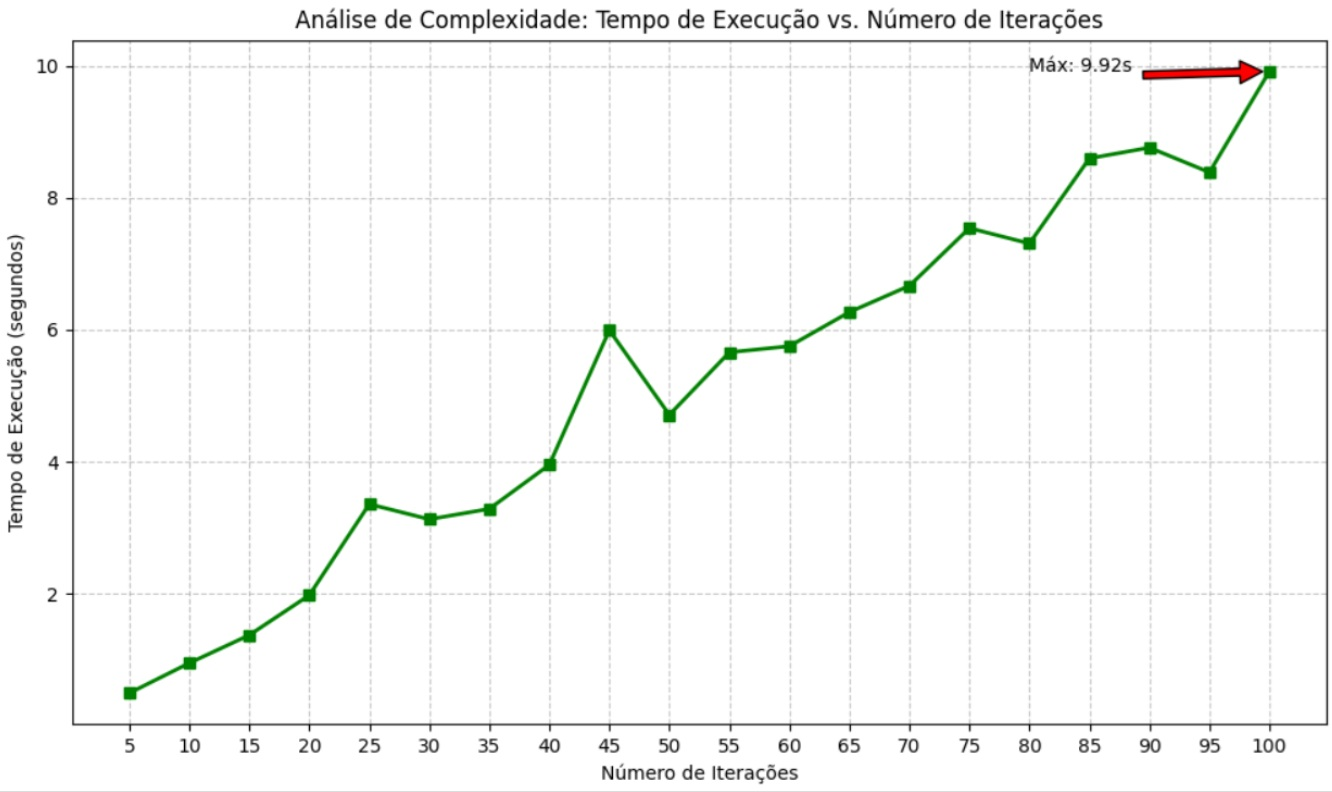
\includegraphics[width=0.75\linewidth]{Imagens/num_iteracoes.jpg}
    \caption{Tempo de execução em função do número de iterações.}
    \label{fig:tempo_iteracoes}
\end{figure}

\section{Resultados}
O algoritmo implementa um menu de opções, onde é possível escolher entre o número máximo de utilizações do mesmo macho para proliferação, podendo ser definido entre 12 à 20 usos máximos. Ao executar o algoritmo, as saídas apresentam o número de formigas, número de iterações, a taxa de evaporação, o tempo de execução do algoritmo e a importância do feromônio e da heurística. Também são apresentados alguns elementos sobre a base de dados utilizadas como o número total de fêmeas, número total de machos, o valor médio e máximo do índice de seleção da prole e o valor máximo de coancestralidade para um determinado conjunto de parâmetros de entradas.
Para fins de análise, levando em consideração que uma metaheurística é um processo probabilístico, ou seja, apenas uma execução não é capaz de verificar a capacidade técnica da solução, foram realizados 30 testes diferentes em cada um dos cenários, onde foram fixados os seguintes parâmetros:
\begin{itemize}
    \item Número de formigas artificiais: 20
    \item Número de iterações: 50
    \item Importância do feromônio \(\alpha\): 1
    \item Importância da heurística \(\beta\): 3
    \item Taxa de evaporação: 0,5
\end{itemize}
Levou-se em consideração que parâmetros mais baixos fazem a colônia nunca aprender padrões à tempo, enquanto números mais elevados aos informados produzem um custo computacional extra no tempo de execução sem ganho significativo dado às soluções, assim, os dados da tabela \ref{resultados_comparativos} apresentam a média dos resultados obtidos após 30 execuções do algoritmo para a entrada de 60 fêmeas e 5 machos.
\begin{center}
\begin{longtable}{|c|c|c|}
\caption{Média dos resultados obtidos após 30 execuções do algoritmo} \label{resultados_comparativos} \\ \hline
\textbf{Limite de uso dos machos} & \textbf{Coancestralidade} & \textbf{Soma dos índices genéticos}\\ \hline
\texttt{12} & 83,32 & 77,50 \\ \hline
\texttt{13} & 83,85 & 82,50  \\ \hline
\texttt{14} & 84,93& 87,50 \\ \hline
\texttt{15} & 85,09 & 92,50 \\ \hline
\texttt{16} & 86,74 & 97,50 \\ \hline
\texttt{17} & 88,44 & 102,50 \\ \hline
\texttt{18} & 91,43 & 107,50 \\ \hline
\texttt{19} & 93,89 & 112,50\\ \hline 
\texttt{20} & 96,21 & 117,50 \\ \hline
\end{longtable}
\end{center}
Os valores da Tabela \ref{resultados_comparativos} mostram que, ao aumentar o limite de uso dos machos, ocorre simultaneamente um agravamento da coancestralidade piorando a qualidade nesse critério já que os machos com maiores índices genéticos individuais poderão reproduzir mais, gerando uma consanguinidade elevada, por outro lado, o aumento do limite de uso também aumenta proporcionalmente a soma dos índices genéticos, melhorando o desempenho produtivo na próxima solução, ao custo de causar possíveis doenças ou fragilidades às gerações futuras. Esse comportamento evidencia uma troca proporcional do problema onde liberar mais acasalamentos por macho favorece soluções geneticamente superiores em termos de mérito, porém às custas de maior concentração genética e, portanto, menor diversidade. Assim, a escolha do limite ideal depende do balanço desejado entre conservação e ganho genético dentro do sistema de seleção. 
Para permitir a comparação equilibrada entre os dois parâmetros avaliados em cada limite $L$, a coancestralidade $C_L$ e a soma dos índices genéticos $S_L$, ambos os valores foram normalizados para o intervalo $[0,\,1]$. A normalização foi realizada segundo
\[
\tilde{x}_L = \frac{x_L - \min(x)}{\max(x) - \min(x)}.
\]

Assim, para a coancestralidade, obtém-se
\[
\tilde{C}_L = \frac{C_L - \min(C)}{\max(C) - \min(C)},
\]
onde $\tilde{C}_L$ representa o custo relativo de cada limite. Como valores maiores de $C_L$ são indesejáveis, quanto mais próximo de $0$ estiver $\tilde{C}_L$, melhor é o desempenho do limite em termos de controle da coancestralidade; inversamente, valores próximos de $1$ indicam pior desempenho.

De forma análoga, para o índice genético, cuja natureza é de maximização, calcula-se
\[
\tilde{S}_L = \frac{S_L - \min(S)}{\max(S) - \min(S)},
\]
onde $\tilde{S}_L$ reflete o ganho genético relativo, com $0$ indicando o pior valor observado e $1$ o melhor entre os limites avaliados.

Após a normalização, a decisão final sobre qual limite é mais vantajoso é realizada por meio da função de utilidade
\[
U(L) = w_S \cdot \tilde{S}_L \;-\; w_C \cdot \tilde{C}_L,
\]
em que $w_S$ e $w_C$ representam os pesos atribuídos ao ganho genético e ao controle da coancestralidade, respectivamente. Quanto maior o valor de $U(L)$, mais vantajoso é o limite $L$, pois isso indica simultaneamente maior ganho genético normalizado e menor custo de coancestralidade normalizada.

Dessa forma, todos os limites avaliados serão submetidos à função de utilidade $U(L)$, que pode ser visualizado na tabela \ref{resultados_normalizados}

\begin{center}
\begin{longtable}{|c|c|c|c|}
\caption{Qualidade dos resultados normalizados para 60 fêmeas e 5 machos} \label{resultados_normalizados} \\ \hline
\textbf{Limite de uso dos machos} & $C_L$ & $S_L$ & $U(L)$\\ \hline
\texttt{12} & 0,000 & 0,000 & 0,000 \\ \hline
\texttt{13} & 0,041 & 0,125 & 0,084\\ \hline
\texttt{14} & 0,125 & 0,250 & 0,125\\ \hline
\texttt{15} & 0,137 & 0,375 & 0,238 \\ \hline
\texttt{16} & 0,266 & 0,500 & 0,234 \\ \hline
\texttt{17} & 0,397 & 0,625 & 0,228 \\ \hline
\texttt{18} & 0,631 & 0,750 & 0,119 \\ \hline
\texttt{19} & 0,822 & 0,875 & 0,053 \\ \hline 
\texttt{20} & 1,000 & 1,000 & 0,000 \\ \hline
\end{longtable}
\end{center}
A análise conjunta da coancestralidade e do ganho genético normalizados evidencia que nenhum limite de uso dos machos é simultaneamente ótimo para ambos os critérios, reforçando a necessidade de uma métrica que avalie o equilíbrio entre custo e benefício. Pela função de utilidade adotada, que privilegia maiores índices genéticos e penaliza incrementos de parentesco, observa-se que o limite \(L = 15\) apresenta o melhor comprometimento entre esses fatores, atingindo o maior valor de \(U(L)\). Para valores abaixo desse limite, o ganho genético cresce lentamente e não compensa a ligeira redução na coancestralidade; para valores acima, embora o índice genético continue aumentando, o crescimento acelerado da coancestralidade gera um impacto negativo proporcionalmente maior. Assim, o limite de \(15\) usos configura-se como mais vantajoso entre os cenários avaliados, oferecendo o equilíbrio mais eficiente entre a preservação da diversidade genética e o progresso genético obtido.

\section{Conclusão}
\label{sec-conclusao}

Neste trabalho, aplicou-se a meta-heurística \textit{Ant Colony System} (ACS) para resolver o problema de acasalamento otimizado em rebanhos, equilibrando simultaneamente dois objetivos conflitantes: minimizar a coancestralidade entre os descendentes e maximizar o ganho genético esperado. A formulação adotada modelou o problema como um grafo bipartido, no qual cada formiga constrói iterativamente uma solução orientada tanto pelo nível de feromônio quanto pela heurística genética, sempre respeitando as restrições reprodutivas impostas aos machos. 

Os experimentos realizados, baseados na média de 30 execuções independentes por cenário, evidenciaram que o aumento do limite de uso dos machos conduz a um ganho genético crescente, porém acompanhado de um aumento igualmente progressivo da coancestralidade. Assim, nenhum limite testado se mostrou simultaneamente ótimo para ambos os critérios. A normalização dos resultados e a aplicação de uma função de utilidade permitiram quantificar o equilíbrio entre custo (coancestralidade) e benefício (mérito genético), indicando que o limite de 15 acasalamentos por macho fornece o melhor compromisso global, oferecendo ganho genético expressivo sem comprometer excessivamente a diversidade.

Conclui-se, portanto, que o ACS é uma abordagem adequada para problemas multicritério de otimização genética no contexto de manejo animal. Além disso, o estudo reforça que a definição do limite de uso dos reprodutores deve considerar não apenas o mérito genético imediato, mas também a sustentabilidade da variabilidade genética ao longo das gerações. Como trabalhos futuros, sugere-se a utilização de funções de utilidade adaptativas, a incorporação de parâmetros econômicos reais, a extensão para múltiplas gerações e a comparação direta com outras meta-heurísticas, como Algoritmos Genéticos e Simulated Anneling, a fim de aprofundar o potencial do ACS em programas de melhoramento animal.


\bibliographystyle{IEEEtran}
\bibliography{Textos/referencias}

\end{document}
